% CVPR 2024 Paper Template; see https://github.com/cvpr-org/author-kit

\documentclass[10pt,twocolumn,letterpaper]{article}

%%%%%%%%% PAPER TYPE  - PLEASE UPDATE FOR FINAL VERSION
\usepackage{cvpr}              % To produce the CAMERA-READY version
% \usepackage[pagenumbers]{cvpr} % To force page numbers, e.g. for an arXiv version

% Import additional packages in the preamble file, before hyperref
%
% --- inline annotations
%
\usepackage[dvipsnames]{xcolor}
\newcommand{\red}[1]{{\color{red}#1}}
\newcommand{\todo}[1]{{\color{red}#1}}
\newcommand{\TODO}[1]{\textbf{\color{red}[TODO: #1]}}
% --- disable by uncommenting  
% \renewcommand{\TODO}[1]{}
% \renewcommand{\todo}[1]{#1}



% It is strongly recommended to use hyperref, especially for the review version.
% hyperref with option pagebackref eases the reviewers' job.
% Please disable hyperref *only* if you encounter grave issues, 
% e.g. with the file validation for the camera-ready version.
%
% If you comment hyperref and then uncomment it, you should delete *.aux before re-running LaTeX.
% (Or just hit 'q' on the first LaTeX run, let it finish, and you should be clear).
\definecolor{cvprblue}{rgb}{0.21,0.49,0.74}
\definecolor{LMUGreen}{HTML}{00883A} % LMU 
\definecolor{LightPurple}{HTML}{969FFF}
\definecolor{Orange}{HTML}{FF8B00}
\definecolor{Pink}{HTML}{FF0090}

\usepackage{url}
\usepackage{pgfgantt}
\usepackage{pgfplots}
\pgfplotsset{compat=1.17} 
\usepackage{multirow}
\usetikzlibrary{fit, arrows.meta, positioning, backgrounds}
% \usepackage{multicolumn}
\usepackage[pagebackref,breaklinks,colorlinks,citecolor=cvprblue]{hyperref}

%%%%%%%%% TITLE - PLEASE UPDATE
\title{\textsc{GiMeFive}: Towards Interpretable Facial Emotion Classification}
% and Classification Using Deep Convolutional Neural Networks

%%%%%%%%% AUTHORS - PLEASE UPDATE
\author{
% For a paper whose authors are all at the same institution,
% omit the following lines up until the closing ``}''.
% Additional authors and addresses can be added with ``\and'',
% just like the second author.
% To save space, use either the email address or home page, not both
% \quad
Jiawen Wang
\qquad
Leah Kawka
\qquad
Mahdi Mohammadi \\
\tt\small\{Jiawen.Wang,Leah.Kawka,Mahdi.Mohammadi\}@campus.lmu.de
}

\begin{document}
\maketitle
\begin{abstract}
    Deep convolutional neural networks have been shown to successfully recognize facial emotions for the past decade in the realm of computer vision. 
    However, the existing detection approaches are not always reliable or explainable, 
    we propose our model GiMeFive with interpretations, 
    i.e., via layer activations and gradient-weighted class activation mapping. 
    % what are the emotion benchmarks? - standardised datasets.
    We compare against the state-of-the-art methods on the facial emotion benchmarks to classify the six basic emotions,  
    namely happiness, surprise, sadness, anger, disgust, and fear. 
    Empirical results show that our model outperforms the previous methods in terms of accuracy. 
    Our code and supplementary material are available at \url{https://github.com/werywjw/SEP-CVDL}. 
\end{abstract}    
\section{Introduction}
\label{sec:intro}

Facial emotion recognition (FER)~\cite{Ko18} is not only an interesting in our daily life, 
but also important in the realm of artificial intelligence and computer vision. 
In this short proposal, 
we aim to leverage several deep neutral networks to analyze and interpret different human facial emotions.

The structure of this report is arranged as follows. 
% \Cref{sec:related} contains the related work of our research. 
In \Cref{sec:approach}, 
we provide the datasets we used, 
the model architecture we implemented, 
and preliminary evaluation results of our model. 
Our code and supplementary material is available at \url{https://github.com/werywjw/SEP-CVDL}.

\begin{figure*}
  \resizebox{\textwidth}{!}{
    \begin{ganttchart}[
      % hgrid,
      vgrid,
      time slot format=isodate,
      x unit=0.3cm, 
      y unit title=0.9cm,
      y unit chart=0.45cm,
      bar height=0.35,
      bar top shift=0.2,
      group right shift=0,
      group top shift=0.1,
      group height=.3,
      group peaks width={0.2},
      milestone left shift=0.5,
      milestone right shift=0.5,
      title label font=\bfseries\Large
  ]{2023-12-21}{2024-02-23}
      \gantttitlecalendar{year, month} \\
      \ganttbar[bar/.append style={fill=LMUGreen}]{Data Collecting \& Processing}{2023-12-21}{2024-01-10} \\
      \ganttbar[bar/.append style={fill=LMUGreen}]{Model Implementing}{2023-12-30}{2024-01-20} \\
      \ganttbar[bar/.append style={fill=LMUGreen}]{Model Training \& Validating}{2023-12-30}{2024-01-20} \\
      \ganttbar[bar/.append style={fill=LMUGreen}]{Report Writing}{2024-01-04}{2024-01-16} \\
      \ganttgroup[bar/.append style={fill=LMUGreen}]{Preliminary Report}{2023-12-21}{2024-01-17} \\
      % \ganttmilestone{Deadline 1}{2024-01-18} \\
      \ganttbar[bar/.append style={fill=Orange}]{Explainable AI}{2024-01-05}{2024-01-18} \\
      \ganttbar[bar/.append style={fill=Orange}]{Model Fine-Tuning}{2024-01-05}{2024-02-07} \\
      \ganttgroup[bar/.append style={fill=Orange}]{Presentation}{2024-01-05}{2024-02-07} \\
      % \ganttmilestone{Deadline 2}{2024-02-08} \\
      \ganttbar[bar/.append style={fill=cvprblue}]{Report Writing}{2024-01-17}{2024-02-22} \\
      \ganttgroup[bar/.append style={fill=cvprblue}]{Final Submission}{2024-01-19}{2024-02-22} \\
      % \ganttmilestone{Deadline 3}{2024-02-23}
      % \ganttlink{elem3}{elem8}
      % \ganttlink{elem2}{elem3}
      % \ganttlink{elem2}{elem4}
      % \ganttlink{elem4}{elem5}
  \end{ganttchart}
  }
  \caption{Overview of the time schedule for the final project}
  \label{fig:schedule}
\end{figure*}

%-------------------------------------------------------------------------
% All authors will benefit from reading Mermin's description of how to write mathematics:
% \url{http://www.pamitc.org/documents/mermin.pdf}.

% Short captions should be centered.



% \begin{figure*}
%   \centering
%   \begin{subfigure}{0.68\linewidth}
%     \fbox{\rule{0pt}{2in} \rule{.9\linewidth}{0pt}}
%     \caption{An example of a subfigure.}
%     \label{fig:short-a}
%   \end{subfigure}
%   \hfill
%   \begin{subfigure}{0.28\linewidth}
%     \fbox{\rule{0pt}{2in} \rule{.9\linewidth}{0pt}}
%     \caption{Another example of a subfigure.}
%     \label{fig:short-b}
%   \end{subfigure}
%   \caption{Example of a short caption, which should be centered.}
%   \label{fig:short}
% \end{figure*}

\section{Approach}
\label{sec:approach}

\subsection{Dataset Aquisition and Processing}
Firstly, 
for all the image data from the training dataset RAF-DB\footnote{\url{http://www.whdeng.cn/raf/model1.html}}~\cite{li2017reliable,li2019reliable}, 
we filter out neutral instances from the original dataset, 
the emotion labels are denoted as 1 (Surprised), 2 (Fearful), 3 (Disgusted), 
4 (Happy), 5 (Sad), and 6 (Angry) for simplicity 
(Our first dataset is downloaded from \url{https://www.kaggle.com/datasets/shuvoalok/raf-db-dataset/code} with the addition csv file to their labels). 
The test result in \Cref{fig:result} is also aggregated from this specific dataset.
To transform and resize the images to \texttt{(64,64)}, 
we convert the images to greyscale with three channels as our original CNN is designed to work with three-channel inputs. 
Also, we randomly flip the images horizontally with a default 50\% chance. 
This kind of augumentation helps in making the model more robust to orientation changes and thus improve the generalization ability. 
Our training dataset is aggregated from CK+~\cite{LuceyCKSAM10}.

\subsection{Model Architecture}
We implemented from scratch an emotion-classification model with four convolution layers at the very begining. 
Following each convolutional layer, 
batch normalization is applied. 
This stabilizes learning by normalizing the input to each layer. 
Then three linear layers are applied to extract features to the final output. 
We also add a \texttt{dropout} layer to prevent overfitting. 
The activation function used after each layer is Rectified Linear Unit (ReLU), 
since it introduces the non-linearity into the model, 
allowing it to learn more complex patterns. 
In order to find the best hyperparameter configuration (see \cref{tab:hyper} for details) of the model, 
we utilize the parameter grid from sklearn~\footnote{\url{https://scikit-learn.org/stable/modules/generated/sklearn.model_selection.ParameterGrid.html}}. 

% model comparison, e.g., SVM try, also VGG
% specific dataset comparison, e.g., RAF-DB & FER+
% Create table for results 

\begin{table}
  \centering
  \resizebox{.47\textwidth}{!}{
  \begin{tabular}{@{}lccc@{}}
    \toprule
    Models &  Accuracy (Vali) &  Accuracy (Test) & Accuracy (Train) \\
    \midrule
    Baseline CNN & 66.3 & 75.2 & 52.6 \\
    ResNet18 & 76.8 & 79.8 & 60.3 \\
    \bottomrule
  \end{tabular}
  }
  \caption{Accuracy (\%) for different models in our experiments}
  \label{tab:model}
\end{table}

\begin{table}
    \centering
    \begin{tabular}{@{}lc@{}}
      \toprule
      Hyperparameter & Configuration \\
      \midrule
      Learning rate & \{0.1, 0.01, 0.001, 0.0001\}  \\
      Batch size & \{8, 16, 32, 64\} \\
      Dropout rate & \{0.5\} \\
      Epoch & \{10, 20, 30\} \\
      Early stopping & \{\texttt{True}, \texttt{False}\} \\
      Patience & \{5\} \\
      \bottomrule
    \end{tabular}
    \caption{Explored hyperparameter space for our model}
    \label{tab:hyper}
  \end{table}

\subsection{Preliminary Results}

For evaluation, we use the metric accuracy. 
The loss function is cross entropy, which is typically for multi-class classification. 
The main results of our experiment with respect to loss and accuracy is depicted in \Cref{fig:result}.

\begin{figure}[t]
  \centering
  % \fbox{\rule{0pt}{2in} \rule{0.9\linewidth}{0pt}}
   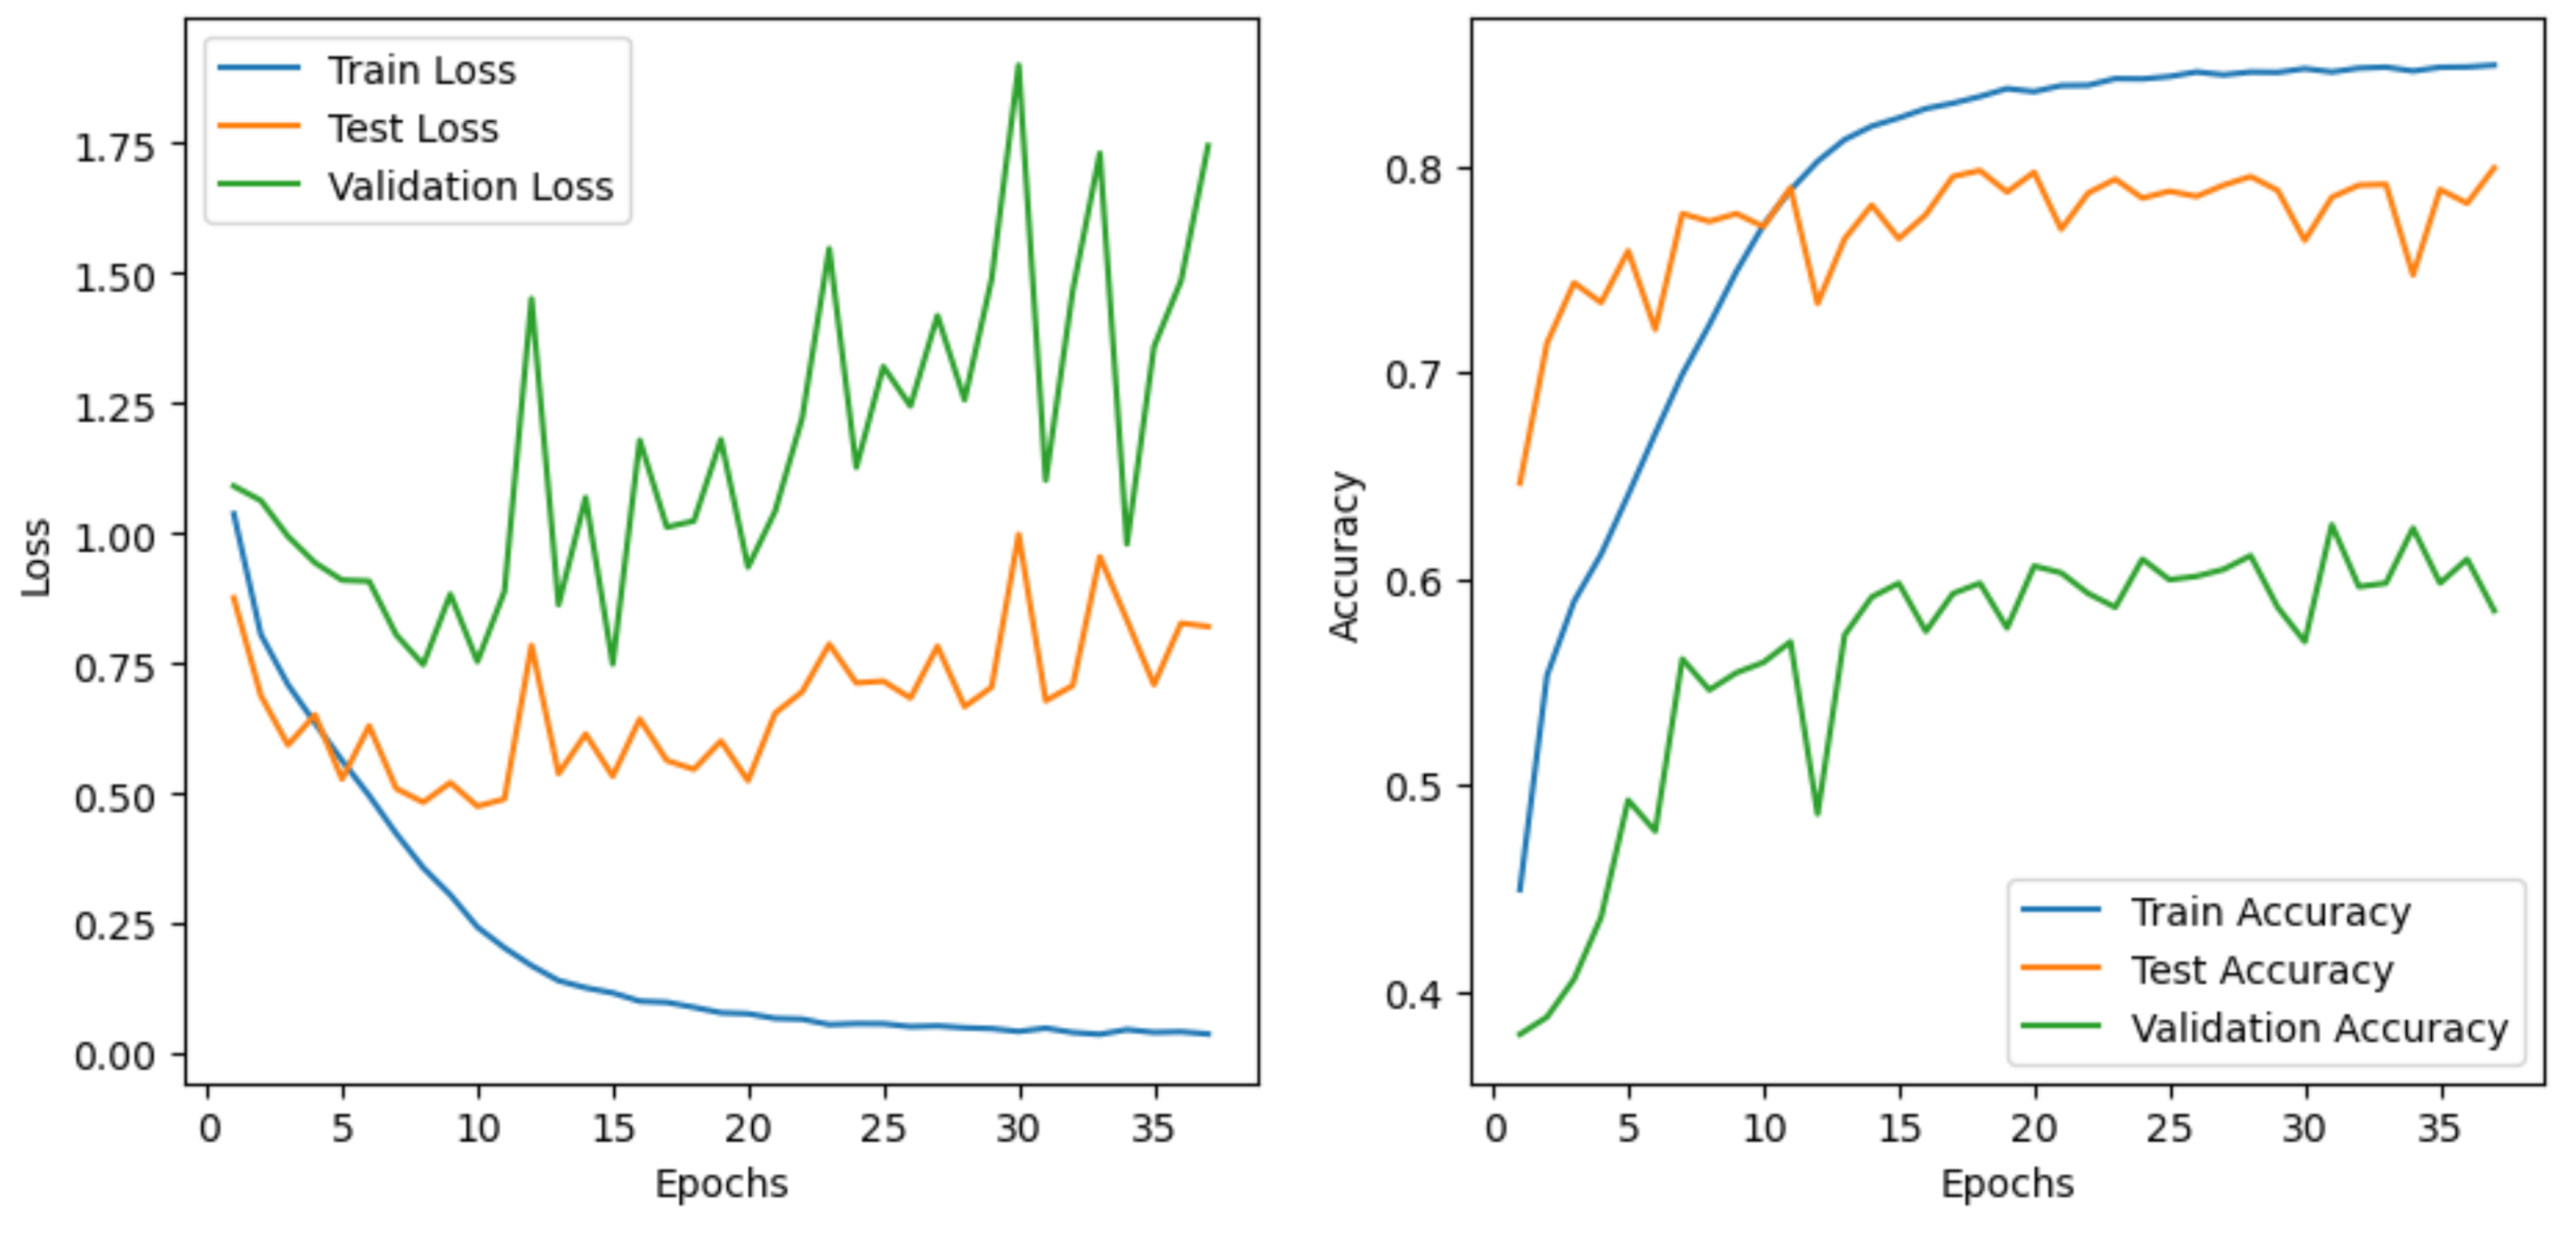
\includegraphics[width=0.95\linewidth]{output.png}
   \caption{Empirical results in terms of the loss and accuracy on differen training epochs}
   \label{fig:result}
\end{figure}

\section{Optimization Strategies}
In the coming weeks, 
we 

\subsection*{Author Contributions}
\label{sec:author}
% see https://arxiv.org/pdf/2005.14165.pdf page42
Equal contributions listed by alphabetical order of surnames. 
Every author did the literature research and contributed to the writing of the paper. 
An overview of our time schedule for the entire final project is given in \Cref{fig:schedule}. 

\begin{itemize}
  \item \textbf{Tanja Jaschkowitz} implemented the model architecture, training and testing infrastructure, 
  \item \textbf{Leah Kawka} collected the training data, prepared dataprocessing, implemented augmentation, run the results, 
  Explainable AI \& Video-green square
  \item \textbf{Mahdi Mohammadi} implemented the 
  \item \textbf{Jiawen Wang} implemented the model architecture, training and testing infrastructure, and optimization strategies. 
  In the specific wrting part, she also checked and aggereated this report from other team members.
\end{itemize}

\section*{Acknowledgements}

We are deeply grateful to our advisors \textbf{Johannes Fischer} and \textbf{Ming Gui} for their helpful and valuable support during the entire semester. 
We also thank \textbf{Prof. Dr. Björn Ommer} for providing this interesting practical course.
\subsection*{Author Contributions}
\label{sec:author}
% see https://arxiv.org/pdf/2005.14165.pdf page42

\begin{itemize}
  \item \textbf{Jiawen Wang} preprocessed the image data 
  and implemented different model architectures including \textsc{GiMeFive}, ResNet18 and 34, 
  and adapted VGG from scratch (with Python, Shell, Markdown, and Jupyter Notebook), 
  training and evaluation infrastructure, classification score and image labeling script, 
  heat-map plot and Grad-CAM explanation, optimization strategies, 
  together with the corresponding writing part. 
  Also, she is responsible for the math, figures, and tables of this report. 
  Besides, she fixed bugs and typo and improved the code/paper quality. 
  \item \textbf{Leah Kawka} collected and managed databases, 
  setup collaborative infrastructure for databases, created a preprocessing script standardize data sources, 
  was involved in training and writing of preliminary and final report, created presentation video, 
  designed architecture of experimental pipeline, coding of augmentation, Grad-Cam and persistence 
  of training results (pickle), implemented slurm/bash script and evaluating script integrating explainable AI 
  (Grad-Cam, Face recognition, Landmarks) to save a video from given video or live camera stream.
\end{itemize}

\section*{Acknowledgements}

We are deeply grateful to our advisors \textbf{Johannes Fischer} and \textbf{Ming Gui} for their helpful feedback and valuable support during the entire semester. 
We also thank \textbf{Prof. Dr. Björn Ommer} for providing this interesting practical course. 

A special acknowledgement to our former team members \textbf{Mahdi Mohammadi}, who joined us till the end of the 
second phase of the project and shared research in conclusion, data pre-processing, and CAM-Images inquiry, 
and \textbf{Tanja Jaschkowitz}, who joined us during the first phase of the project and shared two notebook scripts.
  
% The large face is so funny, not sure where we should put it
\begin{figure}[ht]
  \centering
   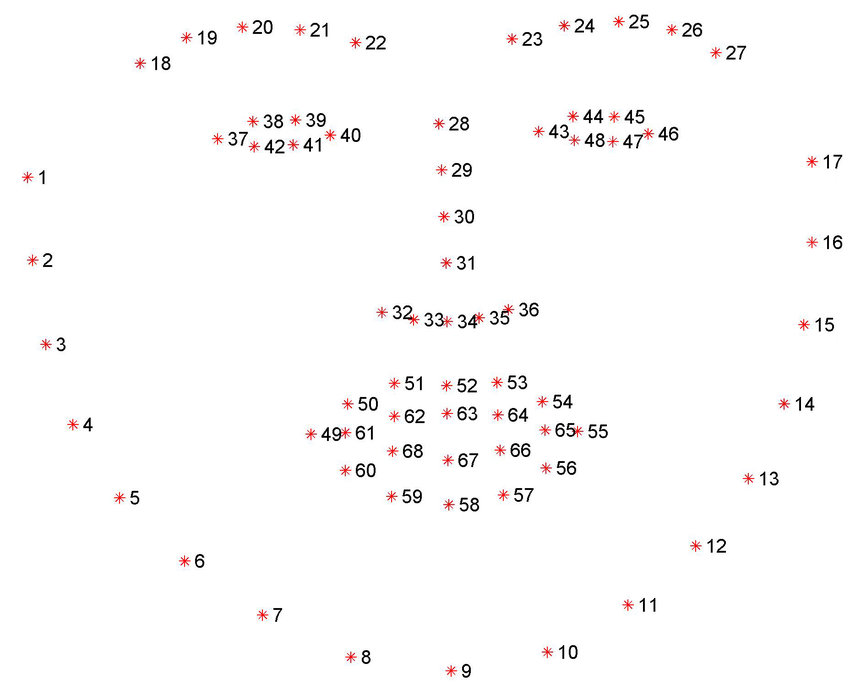
\includegraphics[width=\linewidth]{visual.png}
   \caption{Overview of the confusion matrix on the validation set.} 
   \label{fig:visual}
\end{figure}

\newpage

% \begin{itemize}
%   \item We collected datasets, preprocessed images or videos, 
%   and evaluated the training and testing data thoroughly from various public databases listed in.
%   \item To prepare training and testing images for loading we wrote a script.
%   \item All implemented classification models, such as VGG16, ResNet, 
%   or \textsc{GiMeFive} we built from scratch, 
%   and compared in accuracy in consideration of Layers and Architecture.
%   \item Subsequently optimization was executed with several techniques in a systematic manner. 
%   \item The classification scores of each emotion class, 
%   as well as the parameters to perform the confusion matrix heat map, 
%   are saved (in a serialised PyTorch state dictionary,) with respect to each image or video frame. 
%   \item We provide qualitative benefits such as interpretability to explain our model with Grad-CAM, 
%   combined with Face Landmarks 
%   Landmarks and the indication of the classified emotion percentages, 
%   emphasizing the main emotion.
%   \item To evaluate a video from a given video or live camera we created a script. 
% 	\item To illustrate the real-world performance of our best model \textsc{GiMeFive}, 
%   we edited and provide a demo video.
% \end{itemize}

{
    \small
    \bibliographystyle{ieeenat_fullname}
    \bibliography{main}
}

\subsection*{Author Contributions}
\label{sec:author}
% see https://arxiv.org/pdf/2005.14165.pdf page42

\begin{itemize}
  \item \textbf{Jiawen Wang} implemented different model architectures from scratch, 
  training and testing infrastructure, classification score script, Grad-CAM explanation, and optimization strategies, 
  together with the corresponding writing part. 
  % Also, she is responsible for the figures and tables of this report.
  \item \textbf{Leah Kawka} collected the training data, prepared data processing, and implemented augmentation. 
  She helps run the results with Slurm. 
  She also takes part in the explainable AI and Grad-CAM. 
  In the specific writing part, she drew the %\Cref{}
  \item \textbf{Mahdi Mohammadi} implemented the augmentation, did the research searching, conclusion researching, data preprocessing, and CAM-Images inquiry.
\end{itemize}

\section*{Acknowledgements}

We are deeply grateful to our advisors \textbf{Johannes Fischer} and \textbf{Ming Gui} for their helpful and valuable support during the entire semester. 
We also thank \textbf{Prof. Dr. Björn Ommer} for providing this interesting practical course. 
We especially acknowledge our former team member \textbf{Tanja Jaschkowitz}, 
who joined us during the first phase of the project and shared two notebook scripts.

\section*{Appendix}

\tikzstyle{layer} = [rectangle, rounded corners, minimum width=3cm, minimum height=1cm,text centered, draw=black, fill=LightPurple!30]
\tikzstyle{pool} = [rectangle, rounded corners, minimum width=3cm, minimum height=1cm, text centered, draw=black, fill=cvprblue!30]
\tikzstyle{fc} = [rectangle, minimum width=3cm, minimum height=1cm, text centered, draw=black, fill=Orange!30]
\tikzstyle{arrow} = [thick,->,>=stealth]

\begin{figure}[ht]
  \centering
  \resizebox{.17\textwidth}{!}{
  \begin{tikzpicture}[node distance=1.7cm]

    \node (input) [layer] {Input $3 \times H \times W$};
    \node (conv1) [layer, below of=input] {Conv1 $64$, $3\times3$, padding=1};
    \node (bn1) [layer, below of=conv1] {BatchNorm1 $64$};
    \node (pool1) [pool, below of=bn1] {MaxPool $2\times2$};
    \node (conv2) [layer, below of=pool1] {Conv2 $128$, $3\times3$, padding=1};
    \node (bn2) [layer, below of=conv2] {BatchNorm2 $128$};
    \node (pool2) [pool, below of=bn2] {MaxPool $2\times2$};
    \node (conv3) [layer, below of=pool2] {Conv3 $256$, $3\times3$, padding=1};
    \node (bn3) [layer, below of=conv3] {BatchNorm3 $256$};
    \node (pool3) [pool, below of=bn3] {MaxPool $2\times2$};
    \node (conv4) [layer, below of=pool3] {Conv4 $512$, $3\times3$, padding=1};
    \node (bn4) [layer, below of=conv4] {BatchNorm4 $512$};
    \node (pool4) [pool, below of=bn4] {MaxPool $2\times2$};
    \node (conv5) [layer, below of=pool4] {Conv5 $1024$, $3\times3$, padding=1};
    \node (bn5) [layer, below of=conv5] {BatchNorm5 $1024$};
    \node (pool5) [pool, below of=bn5] {MaxPool $2\times2$};
    \node (adaptivePool) [pool, below of=pool5] {AdaptiveAvgPool};
    \node (fc1) [fc, below of=adaptivePool] {FC1 $2048$};
    \node (dropout1) [fc, below of=fc1] {Dropout $0.5$};
    \node (fc2) [fc, below of=dropout1] {FC2 $1024$};
    % \node (dropout2) [fc, below of=fc2] {Dropout $0.5$};
    \node (fc3) [fc, below of=fc2] {FC3 $6$};

    \draw [arrow] (input) -- (conv1);
    \draw [arrow] (conv1) -- (bn1);
    \draw [arrow] (bn1) -- (pool1);
    \draw [arrow] (pool1) -- (conv2);
    \draw [arrow] (conv2) -- (bn2);
    \draw [arrow] (bn2) -- (pool2);
    \draw [arrow] (pool2) -- (conv3);
    \draw [arrow] (conv3) -- (bn3);
    \draw [arrow] (bn3) -- (pool3);
    \draw [arrow] (pool3) -- (conv4);
    \draw [arrow] (conv4) -- (bn4);
    \draw [arrow] (bn4) -- (pool4);
    \draw [arrow] (pool4) -- (conv5);
    \draw [arrow] (conv5) -- (bn5);
    \draw [arrow] (bn5) -- (pool5);
    \draw [arrow] (pool5) -- (adaptivePool);
    \draw [arrow] (adaptivePool) -- (fc1);
    \draw [arrow] (fc1) -- (dropout1);
    \draw [arrow] (dropout1) -- (fc2);
    \draw [arrow] (fc2) -- (fc3);
    % \draw [arrow] (dropout2) -- (fc3);

  \end{tikzpicture}
  }
  \caption{Overview of our detailed model architecture} 
  \label{fig:modeldetail}
\end{figure}


\tikzstyle{line} = [draw, -latex', line width=0.7pt]

% \begin{figure}[ht]
%   \centering
%   \resizebox{.47\textwidth}{!}{
%   \begin{tikzpicture}[
%     node distance=1cm,
%     auto,
%     rect/.style={rectangle, draw=black, align=center, thick, minimum height=1.5cm, minimum width=2.7cm},
%     box/.style={rectangle, rounded corners, draw=black, align=center, thick, minimum height=1.5cm, minimum width=3cm},
%     bigbox/.style={rectangle, rounded corners, draw=LMUGreen, thick, inner sep=0.3cm, line width=1pt, fill=LMUGreen!5} 
%   ]
%     \node [rect] (data) {Data};
%     \node [rect, below=of data] (mlmodel) {ML Model};
%     \node [rect, below=of mlmodel] (preds) {Predictions};
%     \node [box, right=of mlmodel, fill=cvprblue!30] (interpretability) {Interpretability};
%     \node [box, right=of interpretability, fill=LightPurple!30] (inspection) {Human Inspection};
%     \node [box, below=of inspection] (predictions) {Verified Predictions};

%     \begin{pgfonlayer}{background}
%       \node[bigbox, fit=(data) (mlmodel) (preds)] (group) {};
%     \end{pgfonlayer}
    
%     \path [line] (data) -- (mlmodel);
%     \path [line] (mlmodel) -- (preds);
%     \path [line] (mlmodel) -- (interpretability);
%     \path [line] (interpretability) -- (inspection);
%     \path [line] (inspection) |- node[below left] {Data Improvement} (data);
%     \path [line] (inspection) -- node[left] {Model Improvement}  (predictions);

%   \end{tikzpicture}
%   }
%   \caption{Overview of the traditional standardized ML evaluation process 
%   (see the illustration in the large \textcolor{LMUGreen}{green} box) and the explainable AI pipeline} 
%   \label{fig:xai}
% \end{figure} 

\end{document}
